\section{Learning a default strategy}
\label{sec:part2}
In the previous chapter we created a calculator that can determine the strength of a hand by calculating the probability of winning. In this chapter we shall use the calculator to calculate the strength of the hands.\\

When the APC first joins a poker game it has no information about the opponent, and in this case it must use a default strategy while it gathers more information.

In this chapter we will find a solution to the problem statement:

\vspace{4mm}
\begin{statementBox2}{Problem statement 2}
How can one develop a strategy without having any information about the opponents?
\end{statementBox2}
\vspace{4mm}

Even though players have different strategies they often have some decisions in common. Most players tend to play more aggressively the better their chances are of winning and likewise most players will fold if they have a weak hand. These tendencies can be used in a default strategy. The popular decisions are more likely to be good. For instance, most players agree that it is unwise to fold a pair of aces in the pre-flop. 

The default strategy has to work against every strategy, therefore it is impossible for it to be better than all of them. The goal for the default strategy is not to win, although that is preferable, but instead to reduce the loses while it gathers information about the opponent.

\subsection{Design}
To develop a strategy in poker the two most commonly used options are to either directly program the procedures in the code or to create a self-learning algorithm. 

Programming the procedures in the code requires the programmer to have a deep insight in how to play poker and how to make the optimal decisions during a game. One can also use the expertise of professional poker players in case one lacks the insight.

The self-learning algorithm uses the concept watch and learn by observing other players and trying to learn the strategy behind their decisions. This method requires that the algorithm has someone to observe.

Since we do not have any particular insight in how to play poker and do not have expertise from any professional poker players, we will implement a self-learning algorithm. Additionally, by using this method the computer is not limited by our understanding of the game. We will use data from real life poker games for the algorithm. The data is further described in section \ref{sec:default-test}.\\

To implement the self-learning algorithm we use an artificial neural network (ANN), see section \ref{sec:nn}. The ANN is well suited for finding patterns of the players decisions. 

Our goal is to design an ANN with a total network error (TNE) of five percent or less. We find five percent to be acceptable as players often take irrational decisions and the ANN only tries to find an approximation of the results. 

We use an iterative development method to design the ANN. We start by designing a simple ANN and then move on to more complex ANN's.\\

All our ANN's have exactly two outputs. The first output is whether or not to be defensive by checking or calling and the second output is whether or not to be aggressive by betting or raising. The closer an output is to the value one, the more certain the ANN is, that it is the correct decision. 

All our ANN's use normalised inputs and a sigmoid function as transfer function. The reason we settle for a sigmoid function rather than a step function is because the sigmoid function allows us to see how certain the ANN is of each decision being correct.

\subsubsection{Artificial neural network (ANN)}
\label{sec:nn}
An artificial neural network (ANN) is inspired by the human brain. It can be used for pattern recognition or classification among other things. An ANN can take any number of inputs and return any number of outputs. 

An ANN is made up of neurons that are connected into a network. Each neuron takes a set of inputs and returns a single output. The output of a neuron is sent to all the connected neurons. Each input has a weight that determines influence of the input. The neuron uses an input function to calculate the net input, usually the sum of all weighted inputs, and pass it on to the transfer function. The type of transfer function determines the output. A step function returns zero or one if the net input is above a certain threshold. This is useful for logical functions. If one needs a value between zero and one a sigmoidal function can be used instead.

Figure \ref{fig:neuron} models a neuron. Here the weighted inputs $w_{i1}$, $w_{i2}$, and $w_{i3}$ are all sent to the input function $\sum$ which then calculates the net input $net_{i}$. The transfer function $f$ then calculates the output from the net input.

\begin{figure}[H]
  \center
    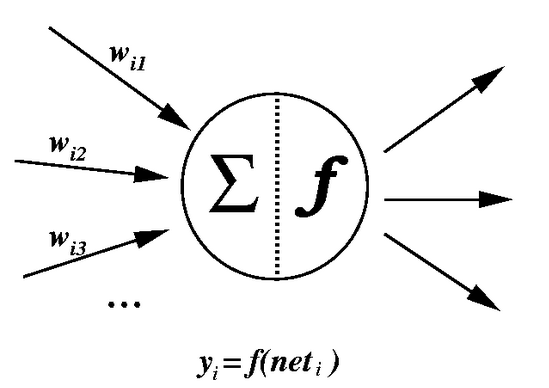
\includegraphics[scale=0.4]{images/nn/neuron.png}
  \caption{Model of a neuron.\cite{neuron} \label{fig:neuron}}
\end{figure}

The neurons in an ANN are distributed in layers as shown in figure \ref{fig:perceptron} and \ref{fig:mlp}. The coloured circles represents neurons and the arrows represents the connections between the neurons. There are three layers, an input layer, a hidden layer, and an output layer. An ANN consists of one input layer and one output layer but may contain any number of hidden layers. The simplest type of ANN is the perceptron which has no hidden layers, see figure \ref{fig:perceptron}. It is used for single calculations. A multilayer perceptron is another type of ANN which contains hidden layers. It is used for more complex domains with multiple layers of computations. 

\def\layersep{2.5cm}

\begin{figure}[H]
\center
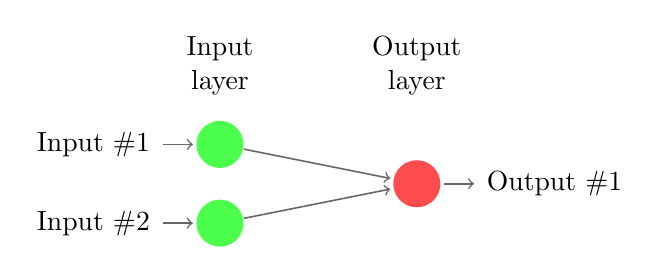
\begin{tikzpicture}[shorten >=1pt,->,line width=0.2mm,draw=black!60, node distance=\layersep]
    \tikzstyle{every pin edge}=[<-,shorten <=1pt]
    \tikzstyle{neuron}=[circle,fill=black!25,minimum size=17pt,inner sep=0pt]
    \tikzstyle{input neuron}=[neuron, fill=green!70];
    \tikzstyle{output neuron}=[neuron, fill=red!70];
    \tikzstyle{hidden neuron}=[neuron, fill=blue!70];
    \tikzstyle{annot} = [text width=4em, text centered]

    % Draw the input layer nodes
    \node[input neuron, pin=left:Input \#1] (I-1) at (0,-1) {};
    \node[input neuron, pin=left:Input \#2] (I-2) at (0,-2) {};

    % Draw the output layer node
    \node[output neuron,pin={[pin edge={->}]right:Output \#1}] (O-1) at (\layersep,-1.5) {};

    % Connect every node in the input layer with every node in the
    % hidden layer.
    \path (I-1) edge (O-1);
    \path (I-2) edge (O-1);

    % Annotate the layers
    \node[annot,above of=I-1, node distance=1cm] (il) {Input layer};
    \node[annot,right of=il] {Output layer};
\end{tikzpicture}
\caption{Perceptron with two inputs and one output. \label{fig:perceptron}}
\end{figure}
\vspace{4mm}
\def\layersep{2.5cm}

\begin{figure}[H]
\center
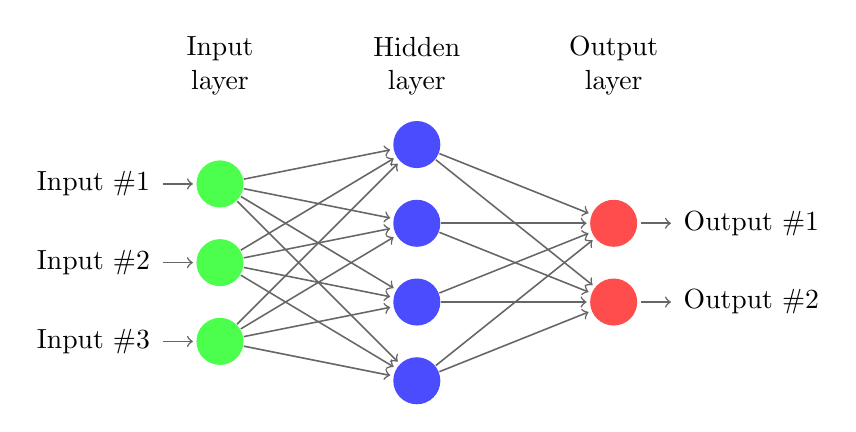
\begin{tikzpicture}[shorten >=1pt,->,line width=0.2mm,draw=black!60, node distance=\layersep]
    \tikzstyle{every pin edge}=[<-,shorten <=1pt]
    \tikzstyle{neuron}=[circle,fill=black!25,minimum size=17pt,inner sep=0pt]
    \tikzstyle{input neuron}=[neuron, fill=green!70];
    \tikzstyle{output neuron}=[neuron, fill=red!70];
    \tikzstyle{hidden neuron}=[neuron, fill=blue!70];
    \tikzstyle{annot} = [text width=4em, text centered]

    % Draw the input layer nodes
    %\foreach \name / \y in {1,...,4}
    % This is the same as writing \foreach \name / \y in {1/1,2/2,3/3,4/4}
    \node[input neuron, pin=left:Input \#1] (I-1) at (0,-1.5) {};
    \node[input neuron, pin=left:Input \#2] (I-2) at (0,-2.5) {};
    \node[input neuron, pin=left:Input \#3] (I-3) at (0,-3.5) {};

    % Draw the hidden layer 1 nodes
    \node[hidden neuron] (H-1) at (\layersep,-1) {};
    \node[hidden neuron] (H-2) at (\layersep,-2) {};
    \node[hidden neuron] (H-3) at (\layersep,-3) {};
    \node[hidden neuron] (H-4) at (\layersep,-4) {};

    % Draw the output layer node
    \node[output neuron,pin={[pin edge={->}]right:Output \#1}] (O-1) at (2*\layersep,-2) {};
    \node[output neuron,pin={[pin edge={->}]right:Output \#2}] (O-2) at (2*\layersep,-3) {};

    % Connect every node in the input layer with every node in the
    % hidden layer.
    \path (I-1) edge (H-1);
    \path (I-2) edge (H-1);
    \path (I-3) edge (H-1);
    \path (I-1) edge (H-2);
    \path (I-2) edge (H-2);
    \path (I-3) edge (H-2);
    \path (I-1) edge (H-3);
    \path (I-2) edge (H-3);
    \path (I-3) edge (H-3);
    \path (I-1) edge (H-4);
    \path (I-2) edge (H-4);
    \path (I-3) edge (H-4);
    
    % Connect every node in the hidden layer with the output layer
    \path (H-1) edge (O-1);
    \path (H-1) edge (O-2);
    \path (H-2) edge (O-1);
    \path (H-2) edge (O-2);
    \path (H-3) edge (O-1);
    \path (H-3) edge (O-2);
    \path (H-4) edge (O-1);
    \path (H-4) edge (O-2);

    % Annotate the layers
    \node[annot,above of=H-1, node distance=1cm] (hl) {Hidden layer};
    \node[annot,left of=hl] {Input layer};
    \node[annot,right of=hl] {Output layer};
\end{tikzpicture}
\caption{Multilayer perceptron with three inputs and two outputs. \label{fig:mlp}}
\end{figure}

The ANN can be trained using a training set of inputs. Using supervised learning, in contrast to unsupervised learning, one must also supply an expected output. For each input it will adjust the weights in order to get closer to the expected output. The TNE indicates the amount of training data that did not produce the expected result. The TNE is calculated during each iteration and the ANN will continue adjusting the weights until the TNE is acceptable. 

Backpropagation is the most common algorithm for supervised ANNs. It adjust the weights from the end (the output neurons) back to the start (the input neurons).

After the training the ANN can be validated to see if it works. This is done using a test set different from the training set and see if the results of the ANN matches the expected results of the test set.

\subsubsection{First ANN design}
\label{sec:design1}
For the first attempt we design a simple perceptron that takes two inputs, and returns two outputs, see figure \ref{fig:nn1}. 
\def\layersep{2.5cm}

\begin{figure}[H]
\center
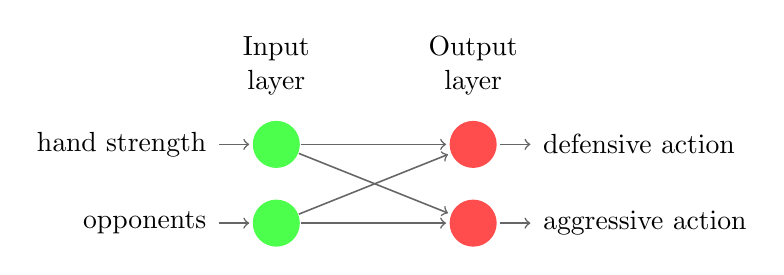
\begin{tikzpicture}[shorten >=1pt,->,line width=0.2mm,draw=black!60, node distance=\layersep]
    \tikzstyle{every pin edge}=[<-,shorten <=1pt]
    \tikzstyle{neuron}=[circle,fill=black!25,minimum size=17pt,inner sep=0pt]
    \tikzstyle{input neuron}=[neuron, fill=green!70];
    \tikzstyle{output neuron}=[neuron, fill=red!70];
    \tikzstyle{hidden neuron}=[neuron, fill=blue!70];
    \tikzstyle{annot} = [text width=4em, text centered]

    % Draw the input layer nodes
    \node[input neuron, pin=left:hand strength] (I-1) at (0,-1) {};
    \node[input neuron, pin=left:opponents] (I-2) at (0,-2) {};

    % Draw the output layer node
    \node[output neuron,pin={[pin edge={->}]right:defensive action}] (O-1) at (\layersep,-1) {};
    \node[output neuron,pin={[pin edge={->}]right:aggressive action}] (O-2) at (\layersep,-2) {};

    % Connect every node in the input layer with every node in the
    % hidden layer.
    \path (I-1) edge (O-1);
    \path (I-2) edge (O-1);
    \path (I-1) edge (O-2);
    \path (I-2) edge (O-2);

    % Annotate the layers
    \node[annot,above of=I-1, node distance=1cm] (il) {Input layer};
    \node[annot,right of=il] {Output layer};
\end{tikzpicture}
\caption{First ANN design. \label{fig:nn1}}
\end{figure}

The first input is the hand strength. We use the calculator from chapter \ref{sec:part1} to calculate the probability of winning against a single opponent. The reason we always find the probability against a single opponent is because the probability of winning decreases drastically as the number of opponents increases. We use an absolute hand strength rather than a hand strength relative to the number of players. This makes it easier to compare the hands strengths in situations with different numbers of players. 

The second input is the number of opponents. The input is normalized as \[I_{norm} = \frac{Opp}{Opp_{max}}\] 
Here $Opp$ is the number of opponents and $Opp_{max}$ is the maximum number of opponents (in our case nine).

From the tests we found that this network had a TNE of $\sim$19,9 \%, see section \ref{sec:ann-test1}. This does not fulfil our requirement of a TNE of five percent or less.

In order for a perceptron to be accurate the data have to be linear separable. This means that the outcomes can be separated by a single line if the are plotted in a graph. We plot some of the data in figure \ref{fig:linear-separable} to see if it is linear separable. The figure clearly shows that the data is not linear separable and therefore a single perceptron will not work.

\begin{figure}[H]
  \center
    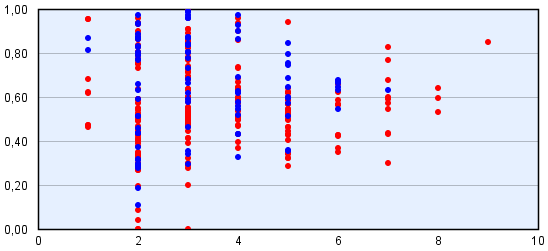
\includegraphics[scale=0.8]{images/nn/default-nn1-plot.png}
  \caption{Distribution of actions. The x-axis  the number of opponents and the y-axis is the hand strength. Aggressive actions are indicated by red dots and defensive actions by blue dots. \label{fig:linear-separable}}
\end{figure}

\subsubsection{Second ANN design}
\label{sec:design2}
Since the first approach designing a perceptron did not fulfil our requirement we instead design a multilayer perceptron (MLP) with five inputs, see figure \ref{fig:nn2}.

The MLP is taking the same inputs as the perceptron from section \ref{sec:design1}, but now it takes three additional inputs: The chips of the player, the cost for the player to call, and the pot. We normalize the three new inputs as: \[I_{norm} = \frac{I}{chips_{total}}\]. 
Here $I$ is the input to be normalized and $chips_{total}$ is the total amount of chips in the game, including the pot and the bets.

The MLP has one hidden layer with two hidden neurons. One hidden neuron to calculate the likelihood of winning and another for the economically aspect.

\def\layersep{2.5cm}

\begin{figure}[H]
\center
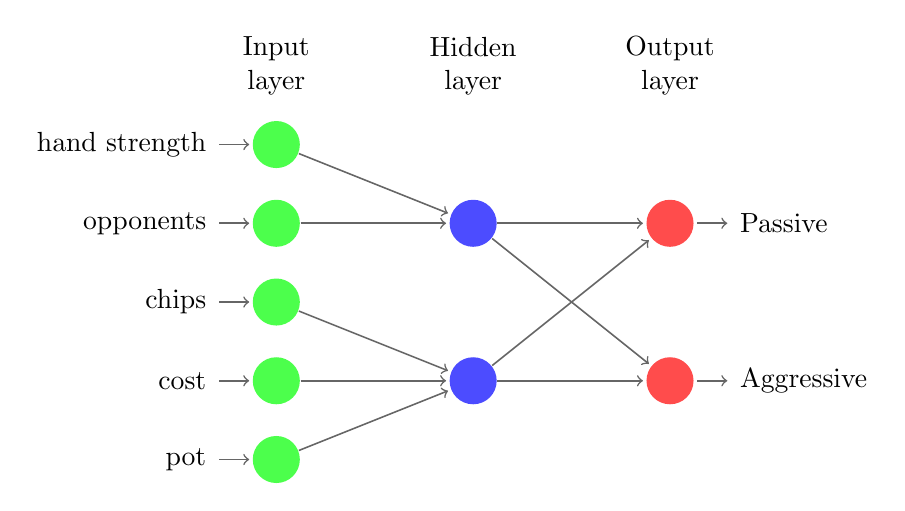
\begin{tikzpicture}[shorten >=1pt,->,line width=0.2mm,draw=black!60, node distance=\layersep]
    \tikzstyle{every pin edge}=[<-,shorten <=1pt]
    \tikzstyle{neuron}=[circle,fill=black!25,minimum size=17pt,inner sep=0pt]
    \tikzstyle{input neuron}=[neuron, fill=green!70];
    \tikzstyle{output neuron}=[neuron, fill=red!70];
    \tikzstyle{hidden neuron}=[neuron, fill=blue!70];
    \tikzstyle{annot} = [text width=4em, text centered]

    % Draw the input layer nodes
    %\foreach \name / \y in {1,...,4}
    % This is the same as writing \foreach \name / \y in {1/1,2/2,3/3,4/4}
    \node[input neuron, pin=left:hand strength] (I-1) at (0,-1) {};
    \node[input neuron, pin=left:opponents] (I-2) at (0,-2) {};
    \node[input neuron, pin=left:chips] (I-3) at (0,-3) {};
    \node[input neuron, pin=left:cost] (I-4) at (0,-4) {};
    \node[input neuron, pin=left:pot] (I-5) at (0,-5) {};

    % Draw the hidden layer nodes
    \node[hidden neuron] (H-1) at (\layersep,-2) {};
    \node[hidden neuron] (H-2) at (\layersep,-4) {};

    % Draw the output layer node
    \node[output neuron,pin={[pin edge={->}]right:Passive}] (O-1) at (2*\layersep,-2) {};
    \node[output neuron,pin={[pin edge={->}]right:Aggressive}] (O-2) at (2*\layersep,-4) {};

    % Connect every node in the input layer with every node in the
    % hidden layer.
    \path (I-1) edge (H-1);
    \path (I-2) edge (H-1);
    \path (I-3) edge (H-2);
    \path (I-4) edge (H-2);
    \path (I-5) edge (H-2);
    
    % Connect every node in the hidden layer with the output layer
    \path (H-1) edge (O-1);
    \path (H-1) edge (O-2);
    \path (H-2) edge (O-1);
    \path (H-2) edge (O-2);

    % Annotate the layers
    \node[annot,above of=I-1, node distance=1cm] (il) {Input layer};
    \node[annot,right of=il] (hl) {Hidden layer};
    \node[annot,right of=hl] {Output layer};
\end{tikzpicture}
\caption{Second ANN design. \label{fig:nn2}}
\end{figure}

From the test in section \ref{sec:ann-test2}, we can see that the TNE is $\sim$19,1 \%. This is a small improvement compared to the first ANN but it still does not fulfil the requirement about a TNE of five percent or less.

\subsubsection{Third ANN design}
\label{sec:design3}
For our first ANN we use the same structure as the second ANN, see figure \ref{fig:nn2}. We believe that the reason the second ANN did not work is because the data is found of random players. Each player may have a different strategy resulting in different actions. This will make it hard for an ANN to find a pattern. 

Instead we use data of a single player in all games the player is relevant. The test in section \ref{sec:ann-test3} shows that the TNE varies quite a bit between the players. The higher the TNE are the harder the player is to predict. Since poker is a game of deception most players will be hard for our ANN to learn.

To further optimise the ANN, we try to adjust the number of hidden neurons, see section \ref{ref:ann-test4}.

\subsection{Test}
\label{sec:default-test}
The University of Alberta has a research group that specializes in the field of artificial intelligence in poker \cite{alberta}. They have released a dataset containing data from $\sim$18.000 real-life rounds of Texas hold'em limit poker. The dataset only contains data about the hole cards of the players who made it to the showdown. We will refer to these players as relevant players.

The dataset consists of multiple files. The file called \textit{hroster} contains the names of all players at the beginning of the round. The file called \textit{hdb} contains the information about the community cards and the flop after each game state. For each player a file called \textit{pdb.}<playername> exists. This file includes the hole cards (if the player did not fold), chips, profit from round and actions during each game state. 

We have collected all the data from the different files into an single data file called \textit{refactored-data.txt} to make it easier to analyse the rounds. We discarded the data for all rounds that has no relevant players. This is because no information about the hole cards exists in such rounds and therefore it is irrelevant for us. 

\textit{refactored-data.txt} will be used for training and testing the ANN's throughout this section.\\

For each test we create a new dataset. This dataset contains the information about the game for each action performed by a relevant player. All informations about the game is found in the moment of the action. For instance, an action in the pre-flop will have no information about the community cards.
Each dataset contains data from 200 random poker rounds, resulting in $\sim$1200 actions distributed across all game states.

To create and test the ANN's we use a framework called Neuroph \cite{neuroph}. Neuroph is a neural network framework programmed in java. 

\subsubsection{Find the TNE of the first ANN}
\label{sec:ann-test1}
For this test the dataset only includes the normalized data about the hole cards of the player, the community cards and the number of opponents.

To find the TNE of the perceptron described in section \ref{sec:design1}, we train it using the dataset. The graph seen in figure \ref{fig:tneg1} displays the TNE through each iteration of the training. From the graph we can see, that the TNE does not get any smaller than $\sim$19,9 \%.

\begin{figure}[H]
  \center
    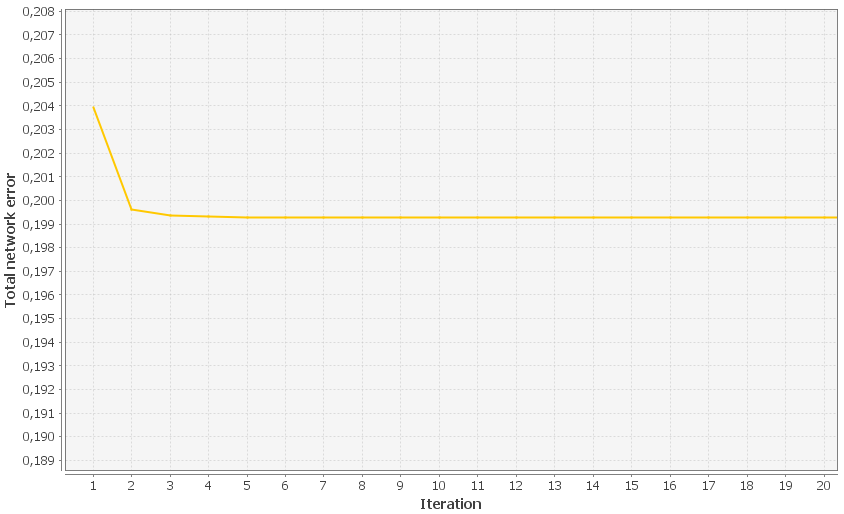
\includegraphics[scale=0.6]{images/nn/default-nn1-err.png}
  \caption{TNE graph from training the first ANN.\label{fig:tneg1}}
\end{figure}

\subsubsection{Find the TNE of the second ANN}
\label{sec:ann-test2}
For this test the dataset also includes the normalised data about chips, cost and pot.

We train the MLP from \ref{sec:design2} and get the NTE graph shown in figure \ref{fig:tneg2}. The TNE does not get any lower than $\sim$19,1 \%.

\begin{figure}[H]
  \center
    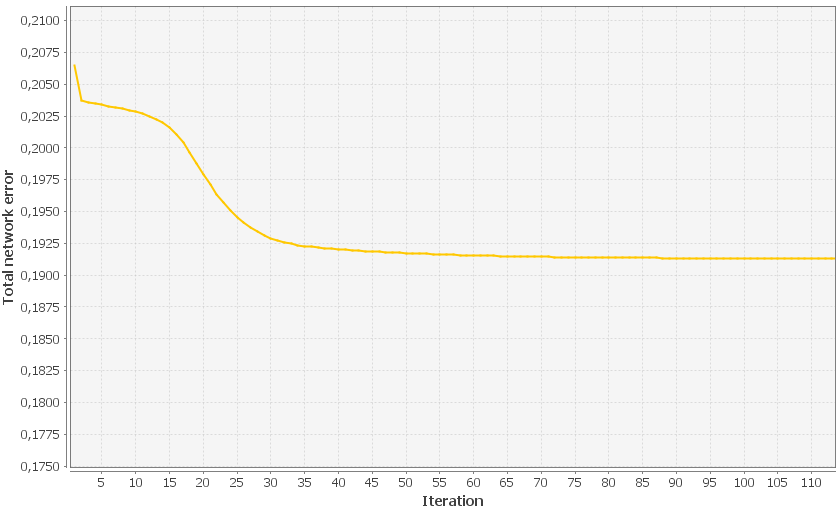
\includegraphics[scale=0.6]{images/nn/default-nn2-err.png}
  \caption{TNE graph from training the second ANN.\label{fig:tneg2}}
\end{figure}

\subsubsection{Find the TNE of the third ANN}
\label{sec:ann-test3}
For this test the dataset contains the same data as the previous test but all data is found for a single player. We try to find the TNE for three different players to see if this makes the ANN more accurate. The players we test are JimR, mayor, and PokiSimA.

For each player we train the MLP from \ref{sec:design3} and find the TNE. The results are shown in table \ref{tab:tneg3}.

\vspace{4mm}
\begin{table}[H]
\center
\begin{tabular}{ | l | l |}
  \hline
  player & TNE (\%) \\
  \hline
  JimR & $\sim$18,7 \\
  mayor & $\sim$14,5 \\
  PokiSimA & $\sim$21,1 \\
  \hline
\end{tabular}
\caption{TNE from training the ANN with different player data.\label{tab:tneg3}}
\end{table}
\vspace{4mm}

\subsubsection{Finding the optimal number of hidden neurons}
\label{sec:ann-test4}

In this test we use the data from the same three player as in section \ref{sec:ann-test3}. We construct three new ANN's with three, five, and seven hidden neurons. The TNE's can be seen in table \ref{tab:tneg4}. We have included the results from section \ref{sec:ann-test3} for comparison. 

The number of hidden neurons does not seem to make the overall TNE get any lower.

\vspace{4mm}
\begin{table}[H]
\center
\begin{tabular}{ | l | l | l | l | }
  \hline
  \#hidden neurons & JimR's TNE (\%) & mayor's TNE (\%) & PokiSimA's TNE (\%) \\
  \hline
  2 & $\sim$19,4 & $\sim$14,5 & $\sim$21,1 \\
  3 & $\sim$19,5 & $\sim$14,0 & $\sim$20,9 \\
  5 & $\sim$19,1 & $\sim$15,0 & $\sim$21,1 \\
  7 & $\sim$17,8 & $\sim$14,9 & $\sim$21,3 \\
  \hline
\end{tabular}
\caption{TNE from training ANN's with different numbers of hidden neurons.\label{tab:tneg4}}
\end{table}
\vspace{4mm}

\subsection{Discussion}
In this chapter we try to develop a default strategy by implementing a self-learning algorithm. We use ANN's to observe actions from other players and learn their strategy. Alternatively, we could have programmed the procedures of determining the action directly in the code. We ran into a few problems by trying to implementing the ANN.\\

The first problem is related to the data we use. The problem is that  the data is not complete since we do not have the data about the hole cards of the irrelevant players. This means that we can not learn the ANN when to fold, as we have no input for the hole cards. To solve this we either need a complete data set or to program the procedure for determining when to fold. 

Additionally, since we get the results as an action (defensive or aggressive), The expected results of each output is either zero or one, due to the limitation of possible actions. These are the two extremes and it can be hard for the ANN to find an approximation.

The second problem was to determine the number of inputs for the ANN. We did not have much luck using only five inputs for our ANN. Since most players adapt their strategy to strategies of the opponents, it is close to impossible to learn the strategy of the player without knowing the strategy of the opponents.

The final problem we encountered was defining our requirements for the ANN. We do know what TNE is realistic and our requirements may be unrealistic. \\

It was a bad idea to try learn a default strategy from random player in random rounds. The players had most likely already gained information about the opponents and thus adapted their strategy to the opponents. It would have made more sense to observe players who just joined a table to see how they played in a situation where they had not adapted to the opponents yet.
Additionally, trying to learn an approximation of every strategy is a bad idea. Observing bad players will cause the default strategy to take bad decisions. It would make more sense to observe only a few successful players. This way we can ensure the decisions to be smart. 

\subsection{Conclusion}
In this chapter we try to answer problem statement 2:

\vspace{4mm}
\begin{statementBox2}{Problem statement 2}
How can one develop a strategy without having any information about the opponents?
\end{statementBox2}
\vspace{4mm}

We develop the strategy by creating an ANN and train it using data from real-life poker games. This solution did not work for us.\\

We trained our ANN to the strategy of random players by observing their actions and the information about the game in the moment of the action. We then found the TNE of the ANN's, and compared them to our requirement of having a TNE of five percent or less. Our best ANN had an TNE of $\sim$14.0~\% and therefore did not fulfil our requirement of five percent or less. 
